%
%
%
%%%%%%%%%%%%%%%%%%%%%%%%%%%%%%%%%%%%%%%%%%%%%%%%%%%%%%%%%%%%

\documentclass[a4paper, 11pt]{report}%choice of the class of the document
\usepackage[french]{babel}%s\'el\'ection du langage
\usepackage{textcomp}%special letter
\usepackage{amssymb,bm,graphicx,graphics,subfigure,geometry}%different packages
\usepackage[breaklinks]{hyperref}
\usepackage[final]{pdfpages}%insertion of pdf
\usepackage{url}%format adress url
\usepackage{fancyhdr}% header and footer can be modified
\usepackage[official]{eurosym}% symbol of money euro. for dollar tape : \$
\usepackage{parskip}% for paragraph and skip

\usepackage[version=3]{mhchem}% for chemistry
\parskip=0.1in% for chemistry
\usepackage[italic]{hepnames} % for proton etc 
\usepackage{mathtools} % for math symbol
\usepackage{amssymb,amsmath}% for insert math eq in latex

\renewcommand\thesection{\Roman{section}} % set own number for section
\renewcommand\thesubsection{\thesection.\Roman{subsection}} % for subsection


%%%%%%%%%%%%%%%%%%%%%%%%%%%%%%%%%%%%%%%%%%%%%%%%%%%%%%%%%%%%
%     few commandes to control geometry of paper :         %
% https://www.sharelatex.com/learn/Page_size_and_margins   %
%%%%%%%%%%%%%%%%%%%%%%%%%%%%%%%%%%%%%%%%%%%%%%%%%%%%%%%%%%%%

\begin{document}

\begin{center}
\bfseries Rapport de stage 3A de mi-parcours\\
\itshape \`a l'intention de M. Sylvain LECLER
\end{center}
 
\section{Pr\'esentation du sujet et calendrier pr\'evisionnel}

  \paragraph{Pr\'esentation du sujet}
  \hspace{1cm}\\ \\
  \indent Pour mon projet de fin d'\'etude, j'ai l'opportunit\' e d'effectuer un stage de recherche \`a TRIUMF, un des plus importants laboratoires nationales 
  du Canada. TRIUMF est situ\' e sur le campus universitaire de l'UBC - University of British Colombia -,  en Colombie Britanique. 
  \\
  Construit en 1971 autour du cyclotron, TRIUMF est sp\' ecialis\' e dans plusieurs th\` emes de recherche de pointe dont celui des particules. Outre sa collaboration 
  avec l'exp\' erience ATLAS au CERN, TRIUMF et nEXO \footnote{next generation Enriched Xenon Observatory.} travaillent ensemble pour mettre en \' evidence la 
  double d\' esint\' egration b\^ eta sans \' emission de neutrinos \(0\Pneutrino\beta\beta\). 
  \\ 
  Si le mod\` ele standard pr\' edit la double d\' esint\' egration b\^ eta avec \' emission de deux neutrinos \(2\Pneutrino\beta\beta\),la mesure de  
  \(0\Pneutrino\beta\beta\)permettra de valider ``la physique au del\'a du mod\` ele standard'', de montrer que les neutrinos ont leur propres anti-particules \footnote{De telles particules sont 
  appel\' ees particule de Majorana} et aussi de mesurer la masse absolue du neutrino. 
  \\
  Parmis les 35 isotopes naturels pouvant produire cette double d\'esint\'egration sans \'emission de neutrinos, le X\'enon \ce{^{136}Xe} est un candidat potentiel.
  L'\'equation ci-dessous conduit \`a l'observation du pr\'ec\'edent candidat \(0\Pneutrino\beta\beta\) :

  \begin{equation}
  \ce{^{136}Xe} \rightarrow \ce{^{136}Ba} + 2\Pelectron \iff 2\Pneutron \rightarrow 2\Pproton + 2\Pelectron \iff \ce{^{136}Xe} \rightarrow 2\APneutrino + 2\Pelectron 
  \end{equation}
   
  \indent Les deux \'electrons sont \'eject\'es avec une energie suffisante pour aller heurter d'autres noyaux \ce{^{136}Xe}. Si un des ces noyaux est heurt\'e, 
  ce dernier passe alors d'un \'etat stable \`a un \'etat exist\'e \ce{^{136}Xe}. En se d\'esexistant, ce noyau \'emet un photon : c'est le processus de 
  scintillation. La longueur d'onde associ\'e \`a cette lumi\`ere de scintillation est de 175 nm - domaine du Vacum Ultra Violet.
  \\
  
  D'ou l'exp\'erience EXO200 puis nEXO : une cuve est remplie de \ce{^{136}Xe} liquide. Les parois de cette cuve sont recouvertes de d\'etecteurs SiPMs 
  \footnote{Silicum PhotoMultiplier.},sensibles aux rayonnements VUV et capable de détecter 1 photon après l'autre (du faite de la taille micrométrique des pixels.
  \\  
  Ainsi ce stage de fin d'\'etude consiste \`a caract\'eriser ces d\'etecteurs SiPMs. Pour cela une lampe flash au X\'enon \' a 175 nm envoit, \`a une certaine r\'ep\'etition, 
  des flashs (photons) sur la surface d'un d\'etecteur SiPM et un oscilloscope affiche le signal provenant de ce dernier. Un ordinateur connect\'e \`a 
  l'oscilloscope permet d'enregistrer le signal observ\'e. Un algorithme permet ensuite de d\'etecter les pulses correspondant \`a la d\'etection d'un photon. 
  
  Un autre \'etudiant et moi m\^eme travaillont \`a la caract\'erisation de ces d\'etecteurs. Je suis responsable de la manipulation de la maquette de travail
  et de l'enregistrement des donn\'ees. Mon coll\`egue de travail est responsable de la programmation de l'algorithme et d'afficher les r\'esultats.
  \\
  La caract\'erisation des d\'etecteurs doit r\'epondre aux \'exigences suivantes : 
  \begin{itemize}
   \item avoir une efficacit\'e \(\geq\)15"\%" \'a 175 nm
   \item avoir un taux de dark noise inf\'erieur \'a 50Hz/mm\texttwosuperior{}
  \end{itemize}
  \vspace*{5mm}
  
  La figure ci-dessous rend comte de la maquette de travail \ref{fig:box} :
  \begin{figure}[!hbtp]
  \centering
  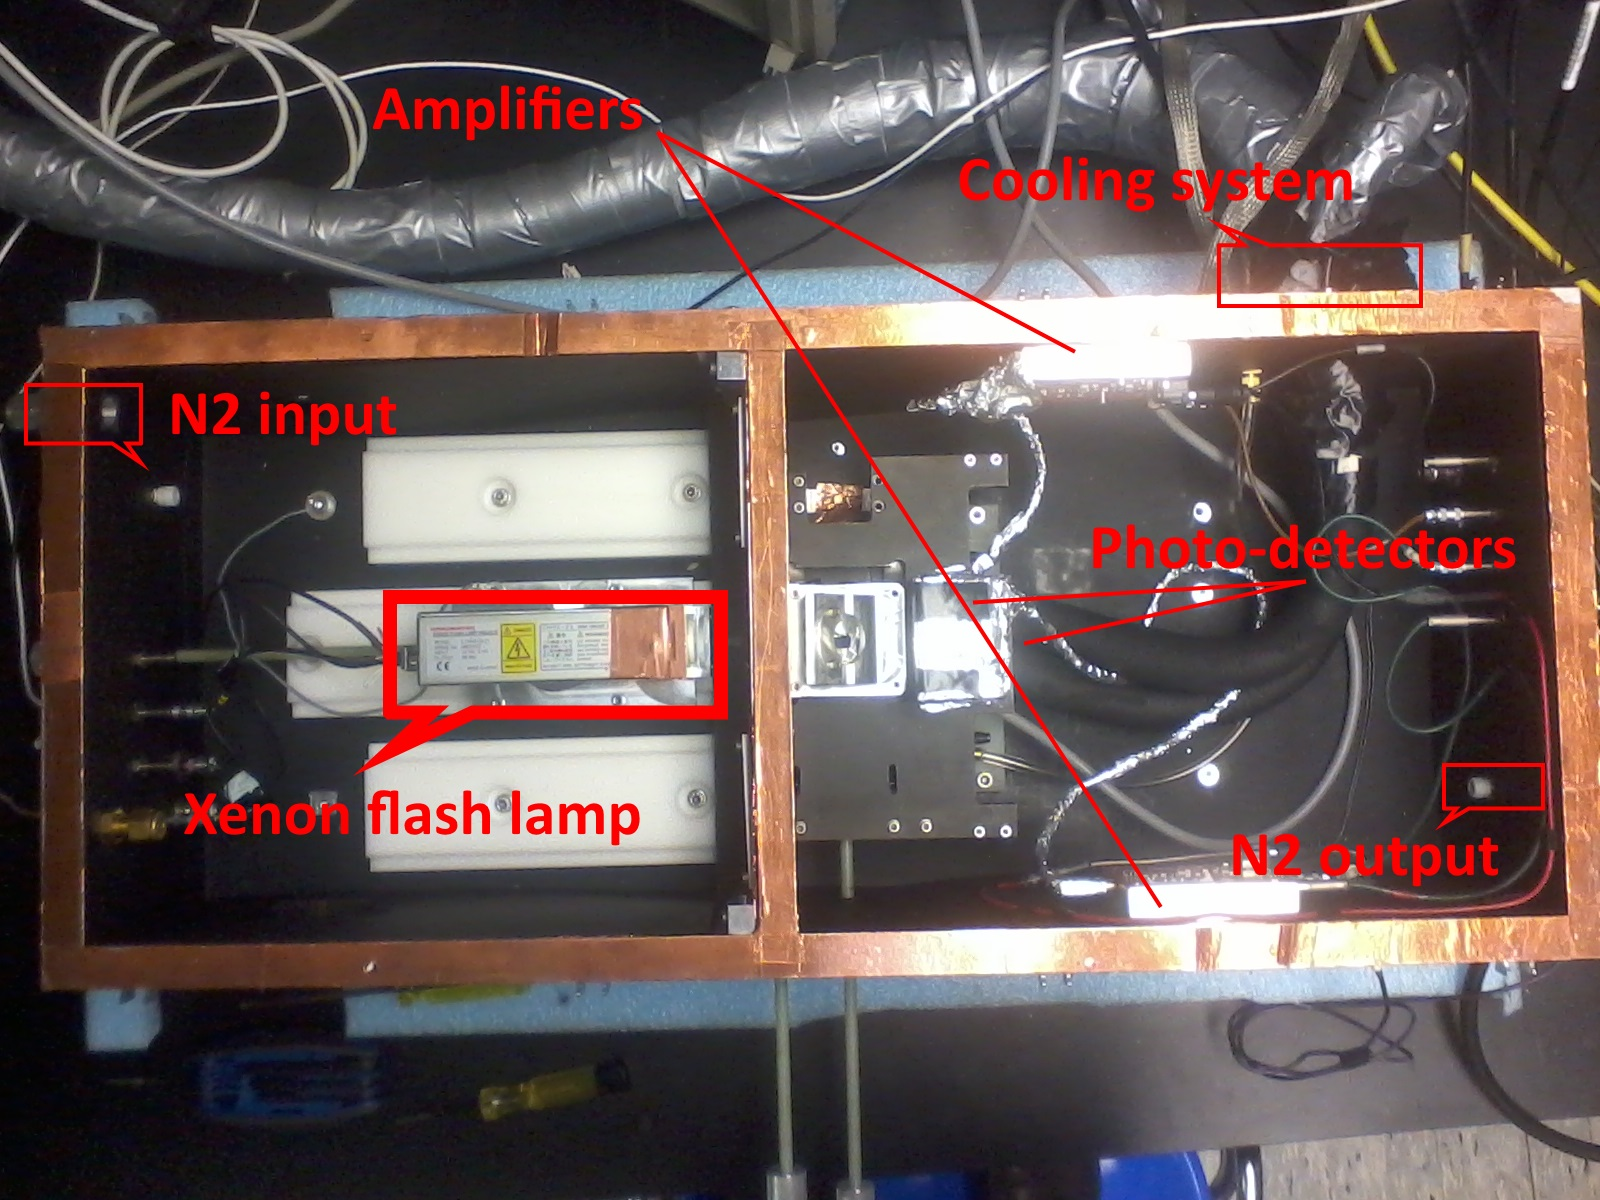
\includegraphics[trim=9cm 1.5cm 4cm 10.1cm, clip=true,totalheight=.45\textwidth]{box.png}%trim=10cm 4cm 1cm 12cm, clip=true, 
  \caption{Partie exp\'eriemental du projet : une boite en aluminium contenant une lampe flash et deux d\'etecteurs SiPMs.}
  \label{fig:box}
  \end{figure}
  
  Le tableau ci-dessous permet de r\'esumer l'avancement de notre travail : 
  
  \paragraph{Calendrier pr\'evisionnel}
  \hspace{1cm}\\ 
  \begin{figure}[!hbtp]
  \centering
  \begin{tabular}{|l|c|c|c|}
  \hline
  D\'etecteur SiPM (diff\'erents fournisseurs) &Efficacit\'e &Dark Noise &Cross Talk + After Pulse\\
  \hline
  MPPC VUV2/MEG &oui &oui &oui\\
  \hline
  MPPC VUV3/MEG &non &non &non\\
  \hline
  MPPC cooted &non &- &-\\
  \hline
  KETEK 1 &- &non &non\\
  \hline
  KETEK 2 & &non &non\\
  \hline
  FDK VUV &non &non &non\\
  \hline
  FBK &- &non &non\\
  \hline
  \end{tabular}
  \end{figure}
  
\section{Plan du projet}
 
  Voici une br\'eve id\'ee du plan qui refletera mon expos\' e lors de ma soutenance.
  \\
  1. Introduction
  \\
  2. Pr\'esentation du laboratoire TRIUMF
  \begin{itemize}
  \item 2.1. Histoire et partenariat
  \item 2.2. Organisation
  \item 2.3. Strat\' egie et th\` emes de recherche
  \item 2.4. L'exp\' eriene nEXO
  \end{itemize}
  3. Pr\' esentation du projet
  \begin{itemize}
  \item La lampe flah au X\'enon. Distribution en temps, ajout de filtres pour att\'enuer la lumi\`ere, mesure de l'attenuation dans l'air et dans 
  le Nitog\`ene gazeux en fonction de la distance de la lampe par rapport aux d\'etecteurs.
  \item Les diff\'erents d\'etecteurs SiPM utilis\'es, leur caract\'eristiques, et la forme d'un pulse associ\'e \' a la d\'etection d'un photon.
  \end{itemize}
  4.  Comptes rendu des activit\'es du stage
  \begin{itemize}
  \item M\'ethodologie de travail
  \item Rapports \'ecrit et conf\'erences audio
  \item R\'esultats
  \\
  - Histrogrammes repr\'esentant la d\'etection de 0 photon, 1 photon etc sur la surface d'un d\'etecteur et comment il est possible d'en extraire 
  l'efficacit\'e. Evolution de l'efficacit\'e des diff\'erents d\'etecteurs SiPM vs tension appliqu\'ee aux bornes de ces d\'etecteurs.
  \\
  - Faire de m\^eme pour le dark noise, le cross talk et l'after-pulse. 
  \\
  - Montrer comment il est possible de reproduire les m\^emes r\'esultats. Pour cela \'etablir et suivre un protocole pour le setup.
  \\
  - Comparer l'efficacit\'e et l'avalanche associ\'ees \`a la d\'etection de photons. Partir des pr\'ec\'edents histogrammes et afficher les graphiques correspondant. 
  \item Discussion des r\'esultats obtenus
  \item Synth\` ese de l'avancement du projet
  \end{itemize}
  5. Bilan professionnel
  \\
  6. Bilan Humain
  \\
  7. Conclusion
  \\
  Bibliographie
  \\
  Terminologie
  \\

\section{Avancement du travail et difficult\'es rencontr\'ees}
 
\paragraph{Avancement du travail}
  \hspace{1cm}\\ \\
  Mon stage ayant officiellement d\'ebut\'e le 09 Mars 2015 j'ai eu trois semaines pour \'etudier la documentation li\'ee au stage. J'ai pu commenc\'e \`a 
  travailler \`a TRIUMF le Lundi 27 Mars.Au regard du calendrier pr\'evisionnel, il est difficile de donner une bonne estimation de l'avancement du travail 
  et cela pour plusieurs raisons. 

\paragraph{Difficult\'es rencontr\'ees}
  \hspace{1cm}\\ \\
  Le principale frein \`a l'avancement du travail vient dans les difficult\'es li\'ees au bruit d'origine \'electromagn\'etique. Ce bruit \'electromagn\'etique
  d\'egrade le signal observ\'e \`a l'oscilloscope. Ainsi les pulses li\'es \' a la d\'etection des photons sont noy\'es dans ce bruit. L'algorithme cr\'e\'e ne peut donc les 
  identifier. 
  \\
  Plusieurs sources de bruit ont \'et\'e identifi\'ees.  

  \begin{itemize}
    \item Les diff\'erents appareils utilis\'es n'avaient pas de masse commune. De ce fait des boucles de courant \'etaient cr\'e\'ees. 
    \\
    La solution a \'et\'e de d'utiliser qu'un seul cable pour mettre \`a la masse ces diff\'erents appareils. 
    \item Quand la lampe flash fonctionne, cette derni\`ere cr\'ee des ondes radios. Ces ondes radios sont capt\'ees par les parties m\'etalliques du d\'et\'ecteur SiPM,
    par l'amplificateur utilis\'e pour amplifier le signal et par le couvercle m\'etallique fermant la boite \ref{fig:box}.
    les solutions on \'et\'e les suivantes : 
    \\- isoler la lampe flash en cr\'eant une cage de faraday recouvrant enti\`erement la premi\`ere partie de la boite, 
    \\- isoler les deux d\'etecteurs des ondes radio en les prot\'egeant avec un papier d'aluminium (cage de Faraday), 
    \\- isoler le couvercle m\'etallique de la boite. Le champ \'electrique provenant de la lampe flash se propageait dans tout le couvercle ce qui pertubait
    le bon fonctionnement des amplificateurs. Des feuilles de cuivre ont permis de guider ce champ \'electrique sur les bords ext\'erieurs du couvercle. 
  \end{itemize}
  \hspace{1cm}\\ \\
  
  De plus l'\'eclairement d\'elivr\'e par la lampe flah faisait satur\'e les d\'etecteurs SiPM. Comme il n'existe pas sur le march\'e de l'optique des filtres 
  pour 175 nm, mes pr\'ed\'ecesseurs ont du les dessiner sous SOLIDWORK. Seulement l'\'eclairement \'etait encore trop fort. La solution a \'et\'e d'utiliser 
  des filtres plastiques. 
  \\
  
  Enfin les retards de livraison des d\'etecteurs ne nous permettent pas de respecter le calendrier pr\'evisionnel. 

\section{Conclusion}

  J'esp\`ere que ce rapport de mi-parcours a donn\'e au lecteur une id\'ee juste de ce en quoi consiste mon travail, de l'avancement du projet et des difficult\'ees
  rencontr\'ees. 
  Lundi 1 Juin, une conf\'erence audio est pr\'evue pour les membres de l'\'equipe nEXO. Elle sera l'occasion de montrer l'avancement du projet. 
  La caract\'erisation de d\'etecteurs SiPM fera l'objet d'une publication. 

\end{document}


remplacer avec Ctrl + R, une fois que le document est fini de r\'edig\'e.
caract\`eres :
'	'
\' a	\'a
\^a	\^a
\'e	\'e
\`e	\`e
\^e	\^e
\`u	\`u
ô	\^o
î	\^i
ï	\\ogi
ç	\c c
œ	\oe{}
²	\texttwosuperior{}
>	\textgreater
``	\og	(ouvrant)
``	\fg{}	(fermant)